% Todo Betere titel vinden
\chapter{Onderzoek: Externe bibliotheken gebruiken en het gevaar hiervan}\label{ch:onderzoek:-SOUP-analyse}
Dit hoofdstuk beschrijft het onderzoek wat gedaan is om meer inzicht te krijgen in het doen van een SOUP-analyse. Als eerst wordt de onderzoeksvraag ontleed in te beantwoorden deelvragen. Daarna zal er wordt iedere deelvraag beantwoord om vervolgens tot een conclusie te komen welke de onderzoeksvraag beantwoord.

\section{Onderzoeksvragen} \label{sec:SOUPOnderzoeksvragen}
De onderzoeksvraag die als startpunt van dit onderzoek geld is:"Hoe kunnen we externe bibliotheken op een veilige manier gebruiken?" of "Hoe kan SOUP op een effectieve manier worden geanalyseerd en hoe maakt dit software veiliger?". Uit deze hoofdvraag kunnen de volgende deelvragen worden ontleed:
\begin{itemize}
    \item Wat is SOUP?
    \item Wat dragen externe bibliotheken en dus ook potentieel SOUP bij aan de ontwikkeling van software?
    \item Wat zijn de gevaren van het gebruik van SOUP?
    \item Wat relateert SOUP tot software veiligheid binnen EagleScience?
\end{itemize}

%Goed verhaal over supplychain Attacks : https://learning.oreilly.com/library/view/alice-and-bob/9781119687351/c01.xhtml#head-2-27

\section{Software of unkown provenance}\label{sec:software-of-unkown-provenance}

\subsection{Wat is Software of Unkown Provenance(SOUP)?}\label{subsec:wat-is-soup?2}
De term SOUP komt oorspronkelijk de wereld van de ontwikkeling van medische software en staat voor "Software Of Unkown Provenance".
SOUP wordt gezien als een software component dat al ontwikkeld is en beschikbaar is gesteld voor gebruik door een instantie anders dan de gebruiker zonder dat de bewijzen zijn over de manier van ontwikkeling als de kwaliteit van de software.
Hierdoor is het dus niet duidelijk welk process er is gevolgt tijdens het ontwikkelen en daarmee dus ook de (medische)veiligheid niet is aan te tonen.
De term wordt nu steeds vaker gebruikt in de algemene software ontwikkel kringen om aan te geven dat er van een betreffent software component(framework, bibliotheek, etc.) niet bekend is hoe het ontwikkeld, getest is.
Hierdoor is er dus geen zekerheid dat het component kwetsbaarheden kan bevatten.
Kwetsbaarheden in deze zin zijn dan voornamelijk lekken of veranderingen van functionaliteiten binnen een software.
\subsection{Hoe relateert SOUP zich met het ontwikkelen van veilige software?}
Om deze vraag te kunnen beantwoorden moeten we eigenlijk twee zaken onderzoeken als eerste  Waarom gebruiken we soup en ten tweede wat wordt er gedaan om veilige software te ontwikkelen.

De voornaamste redenen om bibliotheken te gebruiken is het verminderen van het herhaaldelijk schrijven van code om basis functionaliteiten in een applicatie te krijgen. En Daarmee wordt de ontwikkeltijd verminderd. Het gebruik van bibliotheken is tegenwoordig niet meer weg te denken uit de ontwikkelstrategie van een bedrijf. Deels omdat er een standaard is waarmee gewerkt wordt, wat op zijn beurt het aannemen en opleiden van personeel vergemakkelijkt. Daarnaast hebben veel gebruikte bibliotheken een 'community' waar vragen gesteld kunnen worden om zo moeilijkheden te verminderen. Een nadeel zoals hierboven is beschreven is dat het niet altijd duidelijk is hoe veilig een bibliotheek is.

\section{Veilig software schrijven?}
veilig software schrijven is niet altijd even makkelijk. Er zijn meerdere redenen waarom er niet veilige software wordt geschreven. Tijd en budget zijn vaak de oorzaak omdat software snel op de markt moet komen en er dus niet genoeg tijd gereserveerd wordt om te onderzoeken of er bugs en kwetsbaarheden bevinden. Een tweede mogelijkheid is dat er niet genoeg kennis is om daadwerkelijk veilige software te schrijven. Een andere mogelijkheid is dat er kwaadwillend bewust kwetsbaarheden in bibliotheken worden geschreven om zo een achterdeur te hebben om aanvallen of diefstallen te doen.
In het tweede geval zijn er meerdere instanties die het bouwen van veilige software als doelstelling hebben en er veel aan doen om ontwikkelaars wereldwijd te onderwijzen in goed gebruiken. Eén van de belangrijkste is de OWASP(OWASP.org) de OWASP heeft een aantal projecten die ontwikkelaars in staat stellen om veiligere software te ontwikkelen. Eén daarvan is de OWASP top 20 die ongeveer iedere 5 jaar uitkomt. Dit jaar is er een nieuwe top 10

omlaag brengen van ontwikkeltijd. En het herhaaldelijk moeten schrijven van code. Voor veel basis taken die een applicatie zou moeten uitvoeren is veelal een bibliotheek geschreven die deze taken prima uit kan voeren.


%Bron: "https://johner-institute.com/articles/software-iec-62304/soup-and-ots/"

\section{Hoe kan het gebruik van SOUP gevaarlijk zijn?}\label{sec:hoe-kan-het-gebruik-van-soup-gevaarlijk-zijn?}
Uit een onderzoek van Contrast Security blijkt dat 80\% van de broncode die vandaag de dag gebruikt wordt om een applicatie te schrijven bestaat uit broncode uit een externe bibliotheek.
Waarbij een vierde van de gedownloade bibliotheken kwetsbaarheden bevatten.
De kans dat er dus onbekende kwetsbaarheden in een applicatie sluipen is dus zeker aanwezig.
Een van de redenen dat dit kan gebeuren is een fenomeen dat een package dependency network wordt genoemd.
Wat in het kort betekend dat een dependency die je als ontwikkelaar gebruikt zelf ook een aantal dependencies heeft, welke op zijn beurt ook weer dependecies heeft.
[verder uitwerken]
Dit kan in theorie vele lagen bevatten waardoor de structuur minder inzichtelijk wordt omdat er voor iedere dependency in het netwerk een assesment gedaan moet worden naar kwetsbaarheden.
In verschillende artikelen(Bronnen) wordt gewaarschuwd voor het gevaar van het gebruik deze constructie, echter lijkt het erop dat er binnenkort niet echt verandering komt in de manier waarop dependencies worden gelinkt.
Een andere oplossing zou dan zijn om iedere depenency te checken op kwetsbaarheden tegen een database
Bron: On the inpact of security vulnerabilities in npm package dependency network - Alexandre Decan, Tom Mens, Eleni Constantinou (2018), Structure and Evolution of package dependency networks.

\section{Instanties en SOUP}\label{sec:instanties-en-soup}
Kwetsbaarheden binnen softwareontwikkeling is niet iets van de laatste tijd en er zijn gelukkig instanties die zich bezig houden met het veilighouden van software door middel van trainingen, lezingen en andere manieren van awareness opwekken.
Sommige instanties houden bij welke kwetsbaarheden er gevonden zijn en plaatsen dit in een CVE-database.
Anderen melden veel voorkomende kwetsbaarhden in een top-10

\subsection{CVE Databases, MITRE, NIST, NVD}\label{subsec:mitre-nist-nvd}
CVE staat voor Common Vulenerabilities en Exposures wat een database waarin kwetsbaarheden staan die gevonden zijn in de verschillende systemen.
Deze Database wordt voornamelijk bijgehouden door het bedrijf MITRE dat met subsidie van de US Division of Homeland Security werkt aan het kenbaar maken van lekken in software\footnote{Software wordt hier gezien in de ruimste zin van het woord hierbij hoort: Operating systems, open en closed source software. maar ook frameworks en bibliotheken.}.
De CVE's die in deze database staan worden vervolgens geannalyseerd door het NIST(National Institute os Standards and Technology) en voorzien van een CVSS\footnote{Common Vulnerability Score System is een gestandardiseerde manier om een score aan een kwetsbaarheid toe te kennen waarop in een enkel oog opslag te zien is hoe rieel een risico is.} score en geplaats in de NVD-database.
Zowel de database van MITRE (https://cve.mitre.org) als NIST (https://nvd.nist.gov) zijn publiekelijk toegankelijk.

\subsection{OWASP}\label{subsec:owasp}
Naast het bijhouden van CVE's in database is het creëren van awareness net zo belangrijk.
Een instantie die zich bezig houd hier mee is OWASP(Open Web Application Security Project) die awareness creëert door ideree 5 jaar\footnote{helaas is op het moment van schrijven de laatste versie(2021) nog niet uitgebracht en staat hier de versie uit 2017} een Top-10 uit te brengen met daarin de meest voorkomende en dreigende kwetsbaarheden die ze gevonden hebben in een dataset wat opgebouwd is uit inzendingen van 500+ onderzoekers van 40+ bedrijven die samen meer dan 100.000 API's en web applicaties hebben onderzocht.
In de top 10 die hieronder samengevat weer wordt gegeven wordt er een score meegegeven over hoe makkelijk een lek is te ontdekken en welk mate van risico de kwetsbaarheid heeft.

\begin{figure}[H]
    \myfloatalign
    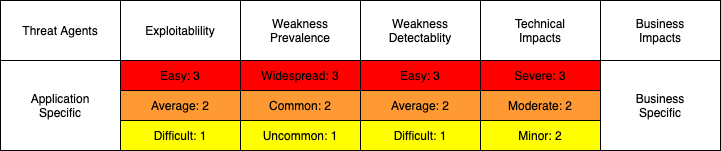
\includegraphics[width=12cm]{gfx/risk tabel}
    \caption{Inschaling van risico's door OWASP}
    \label{fig:risico inschaling}
\end{figure}

\begin{itemize}
%Bron: https://codebros.nl/blog/wat-is-de-owasp-top-10 , https://owasp.org/www-project-top-ten/ << PDF download

    \item \textbf{A01:2017 Injection[exploitabity: 3, Prevelance: 2, detectability: 3, technical: 3]:}

    De mogelijkheid om OS, SQL, NoSQL commandos te injecteren in web applicaties zorgt ervoor dat aanvallers toegang kunnen hebben tot delen van systemen zonder er recht op te hebben.
    Daarnaast is er ook de mogelijkheid om toegang te krijgen tot data die niet voor hen bedoelt is.


    \item \textbf{A02:2017 Broken Authentication[exploitabity: 3, Prevelance: 2, detectability: 2, technical: 3]:}

    Het verkeerd implementeren van authentication en session management kan er voor zorgen dat aanvallers wachtwoorden, sessie tokens aan kunnen passen om zo zich voor te doen als een andere gebruiker.

    \item \textbf{A03:2017 Sensitive Data Exposure[exploitabity: 2, Prevelance: 3, detectability: 2, technical: 3]:}

    Het verkeerd of niet voldoende afschermen van API's kunnen ervoor zorgen dat sensitive data makkelijk gevonden kan worden.\ Zeker als de data niet encrypted verzonden wordt.

    \item \textbf{A04:2017 XML External Entities (XXE)[exploitabity: 2, Prevelance: 2, detectability: 3, technical: 3]:}

    Veel oude of slecht geconfigureerde XML-processoren evalueren externe entiteit referenties binnen XML-documenten slecht.\ Hierdoor is het mogelijk om links te creeën naar bestanden en/of fileshares waar code staat die slecht is voor de applicatie [that contains malicious code].

    \item \textbf{A05:2017 Broken Access Control[exploitabity: 2, Prevelance: 2, detectability: 2, technical: 3]:}

    Beperkingen op wat een geauthenticeerde gebruikers mogen worden niet altijd nageleefd, Aanvallers kunnend deze fouten gebruiken om toegang te krijgen tot gegevens of functionaliteiten die niet bestemd zijn voor deze gebruikers.\ Ze kunnen gegevens aanpassen en / of toegangsrechten aanpassen.

    \item \textbf{A06:2017 Security Misconfiguration[exploitabity: 3, Prevelance: 3, detectability: 3, technical: 2]:}

    Slechte configuratie van de veiligheids instellingen zijn de meest gevonden probleem.\ Dit is meestal het gevolg van het gebruiken van de default, incomplete of ad hoc configuratie Hierdoor kunnen cloud storages open komen te staan, verkeerd geconfigureerde HTTP-headers of foutmeldingen die te veel informatie meegeven ontstaan.

    \item \textbf{A07:2017 Cross-Site Scripting (XSS)[exploitabity: 3, Prevelance: 3, detectability: 3, technical: 2]:}

    Middels XSS is het mogelijk om scripts te draaien van een andere bron dan wenselijk.\ Dit geeft de mogelijkheid om via een browser andere scripts in de applicatie te draaien zo proberen andere functionaliteiten toe te voegen.\ Wat kan leiden tot een web-site dat zich anders gedraagt dan de bedoeling is.

    \item \textbf{A08:2017 Insecure Deserialization[exploitabity: 1, Prevelance: 2, detectability: 2, technical: 3]:}

    Door het niet veilig serialiseren van objecten naar text kan het voorkomen dat er code of commando's mee worden gestuurd welke uitgevoers kunnen worden op de server.

    \item \textbf{A09:2017 Using components with Known vulnerabilities[exploitabity: 2, Prevelance: 3, detectability: 2, technical: 2]:}

    Componenten zoals bibliotheken, frameworks en andere software modules die gebruikt worden voor het ontwikkelen van een applicatie kunnen bedoeld of onbedoeld kwaadaardige code bevatten Wat kan leiden tot verschillende mogelijkheden voor de aanvaller binnen te dringen.\ Of data te versturen naar een andere host om zo achter "beveiligde" gegevens te komen.

    \item \textbf{A10:2017 Insuffivient Logging \& Monitoring[exploitabity: 2, Prevelance: 3, detectability: 1, technical: 2]:}

    Logging en monitoring is bijna net zo belangrijk als het ontwikkelen van een veilige applicatie, mocht er toch een aanval plaatsvinden op welke manier dient er de mogelijkheid zijn om terug te zien wat er precies gebeurt is.\ Logging zorgt hiervoor.\ Het monitoring deel is het bekijken van de logs om te zien of er iets verdachts plaats heeft gevonden.\ Er zijn tools beschikbaar die er voor automatische monitoring zorgen( Nagios is dit soort tool)

\end{itemize}

%Bronnen:
%https://www.imperva.com/learn/application-security/cve-cvss-vulnerability/
%http://owasp.org
\section{Invloed van SOUP op veiligheid van software}\label{sec:invloed-van-soup-op-veiligheid-van-software}
In de OWASP top-10 staat op plaats 9 "Using components with known vulnerabilities" wat aangeeft dat het op het moment van schrijven aandacht nodig heeft.
Eén van de redenen dat dit probleem in de top 10 staat is omdat het gebruik van bibliotheken bijna niet te vermijden is in de ontwikkeling van applicaties wat vooral te danken is aan het steeds sneller moet leveren van een product.
Ontwikkelaars zijn nooit volledig op de hoogte van de werking laat staan wie de onwikkelaar is van een externe bibliotheek.
Een goed voorbeeld hiervan is de "event-stream vulnerability" waarbij de bibliotheek voorzien werd van crypto-coin-stealing malware.
Dit kon gebeuren omdat de bibliotheek niet meer actief werd onderhouden en een persoon zich aanmelde om de ontwikkeling over te nemen.
Vervolgens werd een dependency omgezet van versie en functionaliteit waardoor er toegang werd, verleent om crypto coins te stelen.
Event-stream is een bibliotheek dat veel gebruikt werd als dependency voor applicaties de stream-functionaliteiten van nodejs gebruikten daardoor heeft het de potentie gehad om veel schade aan te richten.
Het is niet geheel duidelijk hoeveel schade er is gelden echter laat dit voorbeeld duidelijk zien wat het probleem is en hoe snel je kan verdwalen in dependency tree's.
Een oplossing is om regelmatig te scannen naar verdachte bibliotheken in de dependency tree.
En er vervolgens actief mee om te gaan door bibliotheken up-to-date te houden.
%Bron: https://www.theregister.com/2018/11/26/npm_repo_bitcoin_stealer/

\section{Dependency trees?}\label{sec:dependency-trees?}
Een dependency tree is een boom structuur waarin staat welke bibliotheken er gebruikt worden door een applicatie en kan beschikken over meerdere lagen.
Laten we als voorbeeld het boven genoemde "event-stream" npm package nemen.
Op de npm website staat vermeld dat deze package ondersteuning biedt aan 1895 andere pakketten en zelf 7 dependencies heeft.
Nu moet je als je zeker wil weten of er kwaadwillende broncode deze ook scannen.
Als we kijken hoeveel dependencies deze weer hebben komen op 4 depenendies die ieders weer dependencies hebben.
De tree van Event-stream is hier te vinden, de kwaadaardige package waar het mis mee ging is verwijderd uit de dependency tree door waarschijnlijk een andere oplossing te vinden.

\begin{figure}[H]
    \myfloatalign
    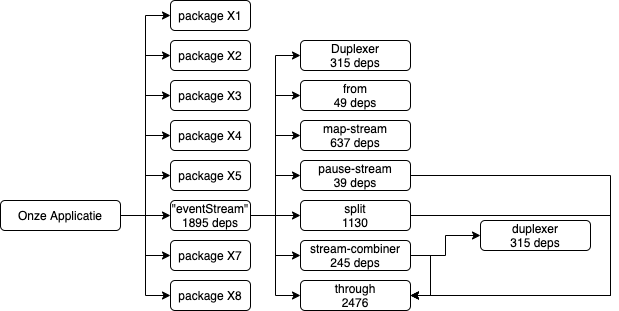
\includegraphics[width=12cm]{gfx/dependency-tree}
    \caption{Dependency tree}\label{fig:dependency-tree}
\end{figure}
Een applicatie heeft niet één zo'n boom maar voor iedere package in de eerste kolom bestaat zo'n boom die dus nog dieper kan gaan dan de hier afgebeelde.
Handmatig scannen is dus geen optie.
Dus moet de oplossing gezocht worden in het autmatisch scannen, gelukkig bestaan er een aantal scanners voor NPM depencies, zxoals versions en retire.js.
Maar ook voor Java en .NET bestaat er een dependency checker ontwikkeld door de OWASP\@.


[NOTE Volgende komt uit SOUP ANALYSE hoofdstuk]

\begin{itemize}
    \item https://jeremylong.github.io/DependencyCheck/
\end{itemize}

Voordat we verder kijken naar mogelijkheden om kwetsbaarheden in een externe bibliotheek te onderzoeken en te verhelpen moeten we eerst kijken naar een aantal kernbegrippen om te begrijpen waar het om gaat.

Dit onderzoek heeft daarom ook twee hoofdvragen die ieders weer een aantal deelvragen opwerpen.
Als eeste is de vraag "Welke kwetsbaarheden bestaan er hoe is het gebruik van externe bibliotheken hier aan gecorreleerd?
De deelvragen die hier uit voorkomen luiden:
\begin{itemize}
    \item Wat zijn applicatie veiligheidsrisico's?
    \item Welke komen het meest voor?
    \item
\end{itemize}

\section{Wat zijn applicatie veiligheidsrisico's}\label{sec:wat-zijn-applicatie-veiligheids-risico's}
Veiligheids risico's binnen applicaties zijn een som van kwetsbaarheden die zich bedoeld of onbedoeld in de applicatie bevinden, de vindbaarheid en de "schade" die er mee aangericht kunnen worden.
De termen van de som worden hieronder verder uitgediept als ook een top-10 uitgeven door de OWASP van de meest voorkomende kwetbaarheden.

Een aanvaller kan op meerdere manier in een applicatie komen(figuur X).
Vaak gebeurt dit door een kwetsbaarheid van een applicatie te zoeken en deze te exploiteren.
Als er vervolgens geen maatregeling genomen zijn om de aanvaller te weerhouden kunnen er zaken als data in een database, assets van het bedrijf of zelfs functionaliteit aangetast worden.
Wat op zijn beurt weer voor een impact in de bedrijfsvoering kan veroorzaken.
Hoe aanvallers een applicatie kunnen aanvallen is applicatie specifiek
De impact op de bedrijfsvoering is ook specifiek
\begin{figure}[H]
    \myfloatalign
    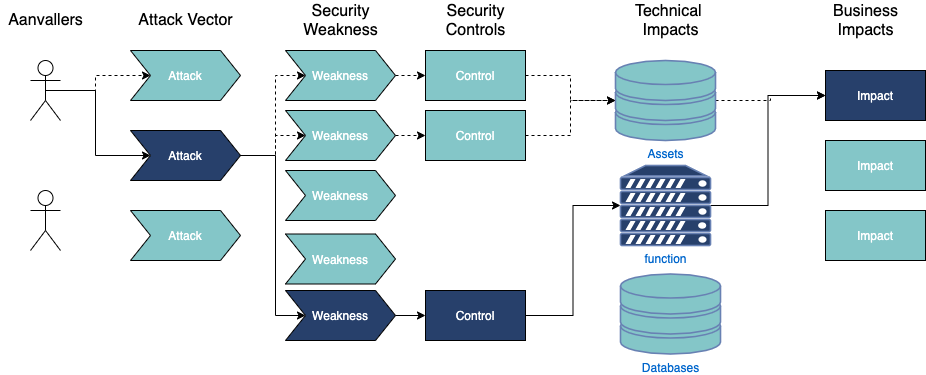
\includegraphics[width=15cm]{gfx/application security routes}
    \caption{Aanvalllen, en hun gevolg}
    \label{fig:Application Security Routes}
\end{figure}

Veiligheids risico's kunnen in categoriën worden geplaatst middels een gradatie systeem die in figuur x te ze zien is.
De OWASP-Top10 die verder in de tekst te vinden is maakt gebruik van dit gradatie systeem om risico's in te schalen.
OWASP is een instantie die zich bezighouden met het verbeteren van de veiligheid van applicaties.
Het doet dit door onder andere training en erkenning te geven aan kwetsbaarheden.
Zo wordt er eens in de 5 jaar een top-10 samengesteld met de op dat moment meest voorkomende kwetsbaarheden.
\footnote{Helaas is de laatste versie die aan het einde van 2021 uit moet komen nog niet beschikbaar op het moment van schrijven}
De OWASP-Top10 wordt samengesteld uit data van meer dan 100.000 productie applicaties en APIs wat door meer dan 500 mensen is getest door 40 verschillende bedrijven.
De top 10 is een aggegratie van deze data in de meest voorkomende issues met inachtneming van exploitabity, detectability en impact.


%\begin{figure}[H]
%  \myfloatalign
%  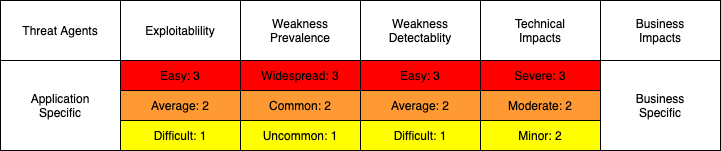
\includegraphics[width=12cm]{gfx/risk tabel}
%  \caption{Inschaling van risico's}
%  \label{fig:risico inschaling}
%\end{figure}

%threat agents = aanvallende entiteit
%exploitabity = exploiteetbaatheid
%weakness prevalance = vookomendheid van de zwakte in een applicatie
%weakness detectability = hoe goed is de zwakte in een applicatie te detecteren
%technical impact = technische impact op de applicaties
%business impacts = (zakelijke impact) impact op de bedrijfsvoering




In het vorige hoofdstuk is te lezen dat Eaglescience gebruik maakt van de volgende technologi\"en: Scala 2.XX, TypeScript, Jenkins, Docker ,Azure cloud.

Dit onderzoek richt voornamelijk op kwetbaarheden in bibliotheken  van derden en de bestrijding ervan.
En specifiek op de bovenstaande door Eaglescience gebruikte technieken.
De hoofdvraag voor dit hoofdstuk luid dan ook: "Met welke kwetsbaarheden hebben we te maken binnen Eaglescience en hoe kunnen we deze opsporen op een automatiseerde manier zonder de huidige werkwijze te verstoren?" Uit deze hoofdvraag onstaan de volgende deelvragen die in dit onderzoek beantwoord worden met daarna een conclusie op de hoofdvraag.

\begin{itemize}
    \item Welke soorten kwetsbaarheden zijn er?
    \item Hoe kunnen deze kwetbaarheden hun weg vinden in onze gebouwde software?
    \item Zijn er instanties die bijhouden waar zich kwetsbaarheden schuilhouden?
    \item Wat zijn methodes om te onderzoeken of er in de bestaande software kwetbaarheden bevinden?
    \item Is er een mogelijkheid om een third-party pakket in te zetten om dit te doen?
\end{itemize}

\

Binnen Eaglescience wordt er heel goed gekeken naar de manier waarop er veilige software ontwikkeld wordt.
Zaken die in de OWASP top-10 staan wordt serieus mee omgegaan en actief tegen gehandeld. zo wordt er ook gegekeken naar het gebruik van bibliotheken van derden.

Op plaats A09:2017 is te vinden dat er kwetsbaarheden middels bibliotheken van derden binnen kunnen komen. Dit is iets wat deels buiten het bereik van Eaglescience ligt. Om ons hier tegen te beschermen is het wenselijk om periodiek en geautomatiseerd een analyse naar kwetbaarheden tedoen.

De bibliotheken die gebruikt worden van derden wordt ook wel Software of unkown pedigree genoemd of kortweg SOUP. Dit houdt in dat een bibliotheek wordt ontwikkeld middels een proces of methode wat niet bekend is bij de eindgebruiker. Ook zijn vaak de details niet bekend van de bibliotheek omdat deze niet of nauwelijks wordt gereviewed door de eindgebruiker. Om deze reden is het dus onbekend of er kwetsbaarheden zitten in betreffende bibliotheken.
De definitie van SOUP blijft niet alleen bij de bibliotheken en frameworks vanuit het open-source gebied. Veelal is ook niet bekend hoe closed-source (Proprietary software) wordt geschreven, echter door reputatie van bedrijven die deze software schrijven wordt veelal , onterecht\footnote{zie: https://www.nu.nl/tech/6097701/waarom-de-hack-bij-solarwinds-ministeries-en-grote-bedrijven-treft.html } aangenomen dat deze geen lekken bevatten.

\section{CVE}
in de appliction security wordt er gesproken van een CVE(Common Vulnerability en Exposures) als een kewtsbaarheid bekend is deze wordt in een database geplaatst zodat \'e\'en ieder die geintreseerd is hier kan vinden welke software(os, applicatie, framework, bibliotheek) mogelijk niet veilig is. Deze Database wordt in stand en bijgehouden door een aantal instanties waarbij de belangrijksten zijn:
\begin{itemize}
    \item \textbf{NIST-CSRC} Computer Security Research Center van het National Institute of Standards and Technology) is een centrum dat onderzoek doet namens de Amerikaanse regering naar veiligheden in software. De database die het NIST-CSRC bijhoud heet het NVD(National Vulnerability Database) waarin CVE's worden bijgehouden.
    \item \textbf{CVE-Mitre} is een community driven effort wat CVE's logt in een lijst die vervolgens de NVD voedt met hun gevondendata.
    \item \textbf{cvedetails.com/}
    \item \textbf{vuldb.com/}
    \item \textbf{https://www.exploit-db.com/}
\end{itemize}

\section{}

https://www.security.nl/posting/666663/Van+CVE+tot+CVSS\%3A+wegwijs+in+het+woud+van+kwetsbaarheden










\section{Zijn er instanties die bijhouden waar zich kwetsbaarheden schuilhouden?}

Naast OWASP zijn er nog een aantal instanties dit bijhouden welke software\footnote{zoals hier gebruikt in de bereedste? zin van het woord dus: (Operating systems, ontwikkeltalen/databases, ontwikkelframeworks,bibliotheken) }
mogelijk kwetsbaarheden kunnen bevatten.
\begin{itemize}
    \item test
\end{itemize}


\section{Wat zijn methodes om te onderzoeken of er in de bestaande software kwetbaarheden bevinden?}

\section{Is er een mogelijkheid om een third-party pakket in te zetten om dit te doen?}
